\documentclass{article}
\usepackage{graphicx}
\usepackage{url}
\usepackage[utf8]{inputenc}

\title{The relevance of Linguistics to Language Technologies}
\author{Sudheer Kolachina}
\date{22/02/2022}

\begin{document}

\maketitle

\section{Introduction}

Language Technologies have seen rapid advances over the last decade. Smart assistants like Siri, Alexa, Google Home and so on, powered by speech and natural language processing are being adopted by millions of users in different locales and languages. This rapid expansion is expected to continue in two main ways- 
\begin{itemize}
    \item Improvement of models for various tasks like Naturalistic Text-to-Speech (TTS), Automatic Speech Recognition (ASR), Spoken Language Translation,  Question-Answering, Conversational AI, Information extraction and so on. 
    \item Expanding the coverage of existing models to new languages (dialects, locales)
\end{itemize}

In this opinion piece, I argue that this ambitious project of building human-like AI cannot be realized without an adequate engagement with linguistics. I demonstrate this using an example from Speech technology where lack of understanding of phonetics-phonology can severely limit our capability to build high quality ASR/TTS models. The overall goal of this article is to raise awareness about the relevance of linguistics to AI and to give pointers to linguists transitioning into the language technologies industry. 
\section{Linguistics and Language technologies: Background}

In this section, I give a brief background on what I mean by linguistics and language technologies. I also discuss a few patterns in previous attempts at collaboration between linguistics and AI. 

Linguistics is the scientific study of Human Language. By human language, we do not refer to any one language but to all human languages. The goal is to develop a theory of how human languages work. There are long-standing debates in different traditions on whether all human languages share some underlying similarities (Universals of Human language) or whether they differ so radically that they endow their speakers with different world views (Sapir-Whorf hypothesis). Regardless of which side of the debate one feels convinced about, one can agree that Human Language is a very sophisticated system with different levels of structure. Figure \ref{fig:linguisticlevels}\footnote{Image source \url{https://commons.wikimedia.org/wiki/File:Major_levels_of_linguistic_structure.svg}} shows the different levels of linguistic analysis. Each concentric circle corresponds to a layer of structure in Human Language. For example, Phonetics is the study of articulation (speaking) and acoustics (hearing) of speech sounds. Similarly, Pragmatics refers to the study of meaning of discourse consisting of multiple sentences, such as conversations, documents and so on. 

\begin{figure}
    \centering
    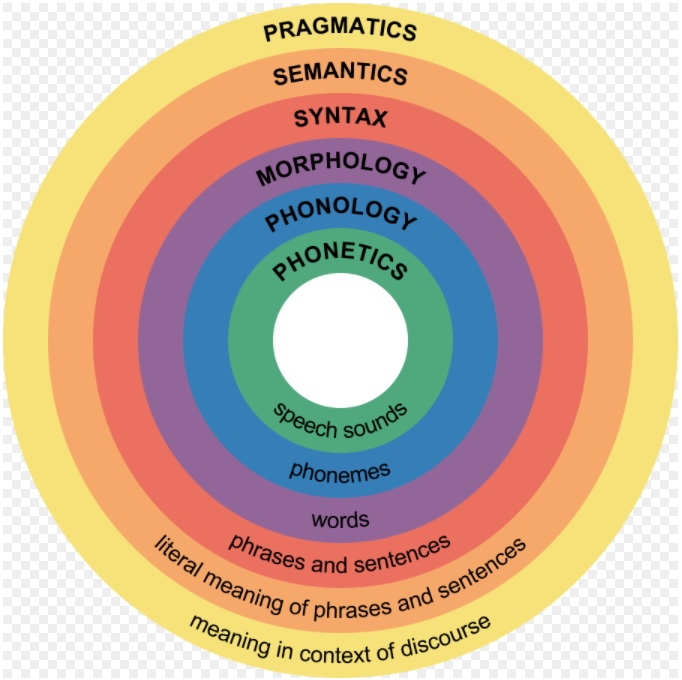
\includegraphics[scale=0.6]{linguisticanalysis.jpg}
    \caption{Levels of Linguistic Analysis}
    \label{fig:linguisticlevels}
\end{figure}

When humans produce a linguistic signal, it contains all these levels of information. In fact, these `levels' were proposed to facilitate understanding of the complex linguistic signal. There is plenty of interaction across levels. For example, you can easily guess the identity of a word whose pronunciation is degraded in an old audio file based on the context of the word. This indicates an interaction between phonetics-phonology and syntax-semantics. In addition, we also rely on visual cues from lip movement, facial gestures and so on while speaking and understanding language (see McGurk effect). Linguists and cognitive scientists have proposed that these visual cues are not separate from Human Language but should be studied as part of Human Language.

Let's examine the goals of language technologies and see if there is any overlap with the levels of linguistic analysis mentioned above. In Figure \ref{fig:langtech}, I show a high level overview of my understanding of Language technologies and its interfaces with various areas of AI. Broadly, Language technologies encompasses the following areas- 
\begin{itemize}
    \item Speech technologies which includes tasks such as ASR, TTS, Speaker diarization, etc. 
    \item Natural Language Processing which includes tasks such as Machine translation, transliteration, Relation extraction, Text paraphrasing, Document Understanding and Summarization and so on.
    \item Knowledge Engineering which includes tasks like Ontology development, building taggers based on ontologies, Knowledge graph engineering, Reasoning using Knowledge Graphs and so on. 
    \item Multimodal processing which includes tasks like Audiovisual processing for Speech, Sign Language recognition, translation and generation and so on. 
\end{itemize}

\begin{figure}
    \centering
    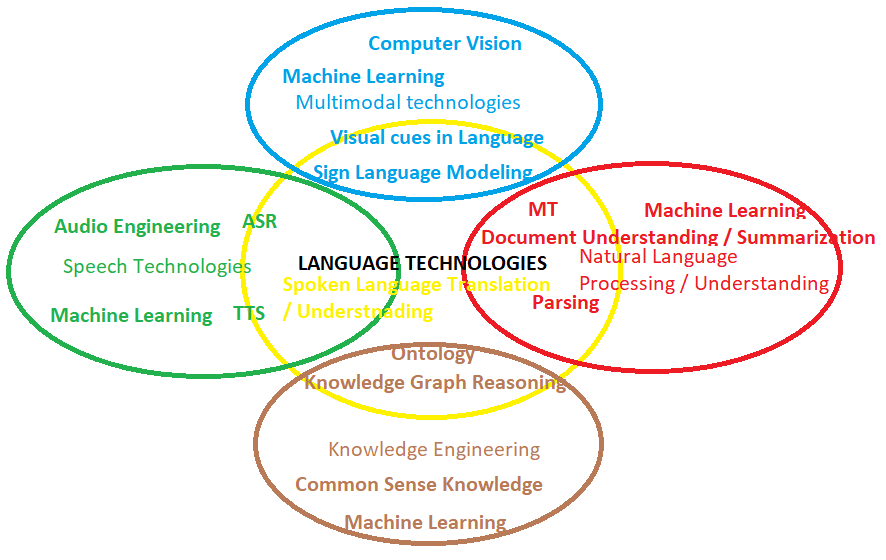
\includegraphics[scale=0.75]{languagetechnologies.png}
    \caption{Language Technologies and AI fields}
    \label{fig:langtech}
\end{figure}

Note that each of these areas contain a machine learning component in the figure. Advances in machine learning models that are unrelated to Language technologies can significantly influence the direction of each of these areas. One example of this is the emergence of deep learning as a result of advances in GPU technology which significantly altered the nature of the solutions in all these areas. Furthermore, each of these areas covers tasks that fall outside the ambit of language technologies. For example, Speech technologies involve a fair bit of Audio engineering- audio compression, speech enhancement, noise reduction and so on which use techniques from Digital Signal Processing and Information theory that can be applied to any kind of signal and are not specific to language. Similarly, multimodal technologies covers areas like computer vision and pose detection which are outside language technologies but can nevertheless help build models of Sign language processing. Certain tasks like Spoken Language Translation or Understanding require significant cross-domain collaboration between Speech and NLP. Similarly, building smart assistants is a very high-level task which involves tasks and techniques from all these areas.

Comparing Figures \ref{fig:linguisticlevels} and \ref{fig:langtech}, we can see connections between different tasks in Language technologies and different levels of linguistic analysis. It is widely accepted that Speech technology is related to phonetics and phonology. However, as mentioned earlier, the linguistic signal is multi-layered and multi-modal and information from syntax-semantics-pragmatics has a significant effect on aspects of speech such as intonation and prosody. Speech technologists have to tackle these aspects if they are to build high quality TTS / ASR systems. Current ASR systems completely ignore intonation, prosody, pitch accents, etc. For example, the text 'It's a beautiful day' has a completely different intonation when spoken as a declarative sentence versus an exclamative sentence. ASR models produce the same output for both these utterances which are linguistically very different. Imagine you are reading a novel and you do not understand the difference between an author declaring and exclaiming (sentiment of surprise) something. Many ASR Engineers in the field are not even aware of these subtle differences in meaning as they are never trained to read articles from linguistics that describe such puzzles of language and seek to solve them. Similar issues exist in TTS. Current TTS models do not fully recognize the rich information conveyed by prosody and intonation in language. These models are often trained on sentence-level training data which is already a bad start as prosody and intonation are related to information structure in the discourse. Again, these terms might sound like Greek and Latin to a TTS Engineer and even to many speech scientists. Before delving into possible reasons for this lack of awareness about linguistics in language technologies, I show in Table \ref{table:taskslevels} different tasks and the level of linguistic analysis they relate to. 

\begin{table}[h!]
\centering
\begin{tabular}{|p{0.6\textwidth}|p{0.4\textwidth}|} 
 \hline
 Task & Level of Linguistic Analysis \\ 
 \hline\hline
 Automatic Speech Recognition, Text-to-Speech, Speaker Diarization, Sentiment analysis from Spoken language & Articulatory and Acoustic Phonetics, Phonology, Prosody, Intonation \\ \hline
 MT, Parsing, Relation extraction Question-Answering, Natural Language Understanding (sentence/document), Text summarization and paraphrasing, Sentiment analysis from text & Syntax, Semantics, Pragmatics \\ \hline
 Ontology development, Knowledge graph & Lexical Semantics, Semantics \\ \hline 
 Audiovisual language processing, Sign Language recognition, production, translation & Syntax, Semantics, Pragmatics, Kinesics  \\
 \hline
\end{tabular}
\caption{Language technologies tasks and how they relate to linguistics}
\label{table:taskslevels}
\end{table}
Now, lets get to the tough part of this discussion. Why are things the way they are? I do not offer any clear answers other than sharing impressions gained over my last $15$ years of experience in linguistics and language technologies. Over the past many decades, there has been an unhealthy competition between linguists and language technologists. Whether it started with Chomsky dismissing the notion of probability of a sentence as 'an entirely useless one' or with computer scientists looking down on linguists as humanities folks who are incapable of objective scientific investigation is anybody's guess. The general consensus in both linguistics and AI is that building theories about Human language and building models that replicate Human language abilities are two different enterprises. Chomsky himself has repeatedly made this distinction between science and engineering and has said that the scientific questions are harder to answer, indirectly implying that the engineering challenges are easier in comparison and thereby, adding to the feeling among language technologists that linguists do not value their work. Another oft-quoted example in this context is Galileo Galilee's studies on flight. Galileo famously tried to build a flying machine based on principles of bird flight he postulated. And failed. This is why many people seem to think studying the scientific principles underlying language might not necessarily help in building smarter language technologies. In my opinion, there are many problems with this analogy- 
\begin{enumerate}
    \item 
    %A Flying machine has no requirement that it should fly similar to a bird or any species that can fly. While a language technology bot needs to speak and understand Human language. 
    %Galileo (among others) tried to apply principles underlying bird flight to build a flying machine. The goal of such attempts was to create machines with the ability to fly which is a property shared by many species in nature.
    Human language ability is different from flight in that it is unique to Humans. The goal of language technologies is to build machines that can understand and produce Human speech. A perfect TTS model for a language should be indistinguishable from a fluent native speaker. On the other hand, a flying machine has no requirement that it should fly similar to a bird or any other species capable of flight.
    
    \item Whether Galileo failed in his goal to build a flying machine or not is a question for experts on history of science. But, in science, most of us will agree that failure is more common than success. Failure is not a reason to give up on studying something. It is likely that efforts to apply insights from linguistics in language technology might not show immediate success. But, in the long run, they can contribute to a richer understanding of the linguistic signal in Speech and NLP models and thus, advance the quality of thought in the field of AI. 
    
    \item It is also worth thinking about what we mean by `applying principles' underlying a phenomenon in an engineering task. Scientific theories are always in flux and we seldom have any certain answers. This is especially true of cognitive sciences where humanity has only uncovered the tip of the iceberg. Principles of linguistics (or bird flight) might not directly solve engineering problems but can help formulate or refine understanding of a problem to the point where an efficient engineering solution emerges.
\end{enumerate}

In my opinion, a better example of the interaction between scientific and engineering goals is that of the steam engine. The nineteenth century French engineer Nicholas Carnot, while working on developing the steam engine, observed that converting heat into work was significantly less efficient than converting work into heat. This is because heat escapes into the environment making $100$ percent conversion to work infeasible. Based on this observation, Carnot formulated a generalization that energy always flows from a higher \textit{entropy} system to a lower entropy system. Years after Carnot's death, this observation led to the development of the second law of thermodynamics. This example is extremely pertinent for linguists who see the engineering project of language technologies as completely unrelated to the goal of building linguistic theories.

\section{Phonetics-Phonology in Speech technology}

In this section, we look at a concrete example from Speech technology on the relevance of phonetics-phonology.
\begin{enumerate}
    \item In TTS, when you build a voice for let's say, Spanish, the model needs to handle English words in the input text. English movie, place and person names are common examples of foreign language tokens in code-mixed speech. The TTS model is expected to pronounce these words in the same way a native speaker of Spanish pronounces them. One way of solving this problem is to get such code-mixed data recorded by native speakers and train your model on such data. But, such data is often not readily available and is very expensive to obtain. In such scenarios, engineers have to resort to creative solutions like mapping the phone sequence of the English word to a phone sequence likely to be produced by the Spanish native speaker. This is, as we will see, a non-trivial task which requires significant understanding of phonetics, phonology and the distinction between the two.
    \item Researchers in ASR/TTS try to leverage TTS models of resource-rich languages to build ASR/TTS models for low resource languages. Again, one of the challenges in such projects is to map the phone set of the low resource language to the phone set of the high resource language. As we will see, this is quite a tricky problem. 
\end{enumerate}
   
\begin{table}[h!]
\centering
\begin{tabular}{|p{0.2\textwidth}|p{0.8\textwidth}|} 
 \hline
 \textbf{Phone} & \textbf{Articulatory features} \\ \hline 
    M & $+$bilabial,$+$nasal \\ \hline
    P & $-$voice,$+$bilabial,$+$stop \\ \hline
    B & $+$voice,$+$bilabial,$+$stop \\ \hline
    F & $-$voice,$+$labiodental, $+$fricative \\ \hline
    V & $+$voice,$+$labiodental,
    $+$fricative \\ \hline
    TH & $-$voice,$+$dental,
    $+$fricative \\ \hline
    DH & $+$voice,$+$dental,
    $+$fricative \\ \hline
    N & $+$alveolar,$+$nasal \\ \hline
    T & $-$voice,$+$alveolar,$+$stop \\ \hline
    D & $+$voice,$+$alveolar,$+$stop \\ \hline
    S & $-$voice,$+$alveolar,$+$fricative \\ \hline
    Z & $+$voice,$+$alveolar,$+$fricative \\ \hline
    R & $+$alveolar,$+$approximant \\ \hline
    L & $+$alveolar,$+$lateral \\ \hline
    SH & $-$voice,$+$palatal,$+$fricative \\ \hline
    ZH & $+$voice,$+$palatal,$+$fricative \\ \hline
    Y & $+$palatal,$+$approximant \\ \hline
    NG & $+$velar,$+$nasal \\ \hline
    K & $-$voice,$+$velar,$+$stop \\ \hline
    G & $+$voice,$+$velar,$+$stop  \\ \hline
    W & $+$labiovelar,$+$approximant \\ \hline
    HH & $+$glottal,$+$approximant \\ \hline
    CH & $-$voice,$+$alveolar,$+$stop,$+$fricative \\ \hline
    JH &  $+$voice,$+$alveolar,$+$stop,$+$fricative \\ \hline
    AO & $-$high, $+$mid, $+$back,  $+$round,$+$vowel \\ \hline
    AA & $-$high, $+$back, $-$round,$+$vowel \\ \hline
    IY & $+$high,$-$back, $-$round,$+$vowel \\ \hline
    UW & $+$high, $+$back, $+$round,$+$vowel \\ \hline
    EH & $-$high, $+$mid,$-$back, $-$round,$+$vowel \\ \hline
    IH & $+$high,$-$tense,$-$back, $-$round,$+$vowel \\ \hline
    UH & $+$high,$-$tense,$+$back, $+$round,$+$vowel \\ \hline
    AH & $+$mid, $+$central, $-$round,$+$vowel \\ \hline
    AE & $-$high,$-$back, $-$round,$+$vowel \\ \hline
    EY & $-$high, $+$mid,$-$tense,$-$back, $-$round,$+$vowel \\ \hline
    AY & $-$high,$-$back, $+$central,$-$round,$+$vowel\\ \hline
    OW & $+$high, $+$mid, $-$tense, $+$back, $+$round, $+$vowel \\ \hline
    AW & $-$high, $+$back, $+$central, $-$round, $+$round,$+$vowel \\ \hline
    OY & $-$high, $+$mid, $+$back,$-$back,$+$round, $-$round,$+$vowel \\ \hline
    ER & $+$high, $+$mid, $+$central, $+$rhotic,$+$vowel \\ \hline
\end{tabular}
\caption{Articulatory features of phones from CMU dictionary}
\label{table:phonefeat}
\end{table}

\begin{figure}[h!]
    \centering
    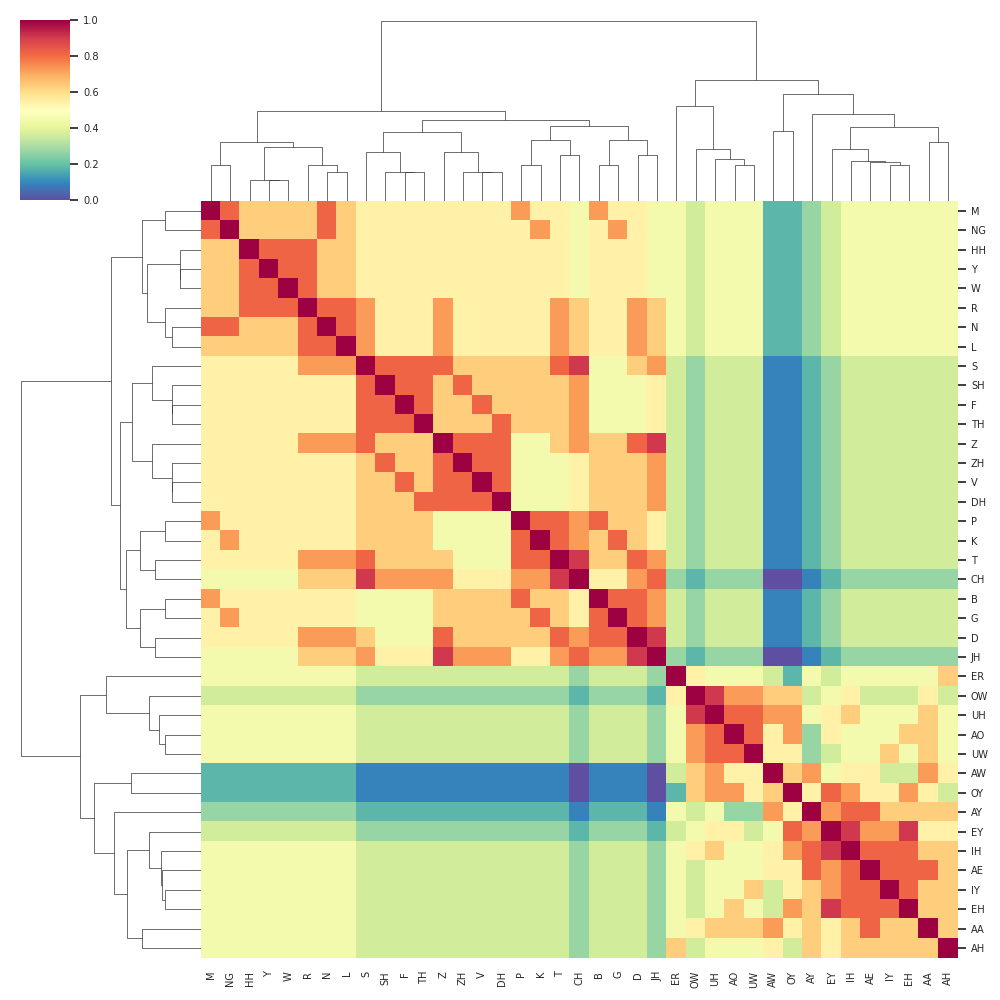
\includegraphics[scale=0.5]{phone-featuresimilarity.png}
    \caption{Phone classes of English based on Phonetic similarity}
    \label{fig:phonsim}
\end{figure}

The most common strategy to map between phones across languages is the `closest phone' approach. That is, for problem $1$ above, each phone in the English word is mapped to the most similar phone in Spanish. For problem $2$, similarly, each phone in the low-resource language is mapped to the most similar phone in the high resource language. Note how this approach relies on a notion of similarity between phones. How is this similarity defined and estimated? Most papers and engineers I came across think of phone similarity in terms of articulatory (or acoustic) similarity. As we will see in the rest of this section, this definition of similarity is incomplete.

Even the notion of articulatory similarity relies on articulatory features of phones developed over the decades by linguists. Each phone can be defined as a bundle of features based on its articulatory characteristics. In table \ref{table:phonefeat}, I show the feature specification of different phones in the phone set of the CMU pronunciation dictionary for English. The similarity between two phones can be estimated as the percentage of common features (Jaccard similarity index). If we cluster these phones based on this similarity, we get the phone classes shown in Figure \ref{fig:phonsim}. As shown in the figure, vowels and consonants form separate clusters. Within each of these clusters, there are different sub-clusters. For example, back vowels OW, UH, AO, UW form a separate cluster as do the front vowels EY, IH, AE, IY, EH. Similarly, within the class of consonants, the voiceless fricatives S, SH, F, TH form a cluster distinct from the voiced fricative Z, ZH, V, DH. 

Everything looks good and seems to make sense. Except for one crucial point. This notion of phone similarity completely ignores phonotactics - in other words, the contexts in which phones occur. If we were to estimate similarity between phones based on the contexts they occur in, would we end up with a similar heatmap? We can test this by training a Transformer language model and estimating similarity between the phone embeddings learnt by the model. In Figure \ref{fig:contsim}, the phone classes of English estimated by applying hierarchical clustering to a distance matrix of Euclidean distances between phone context embeddings are shown. These clusters look similar to the clusters based on articulatory features. However, they are not identical. Vowels and consonants form two separate clusters. Within the class of vowels, the front vowels and back vowels do not form separate clusters as in Figure \ref{fig:phonsim}. Rather the clustering among vowels are based on the similarity of their contexts. Within the class of consonants again, the clusters are very different from the ones based on articulatory features. Voiceless stops P, T, K form a cluster while voiced stops B, D, G form another cluster. Interestingly, the voiceless fricative F seems to cluster with the voiced stops. The affricates CH, JH and the fricatives ZH, DH, TH, V, SH cluster together. The glides Y, W form another cluster. All these clusters make sense to a phonologist as these consonants form \textit{natural classes}. In fact, the goal of distinctive feature specification of phones is to capture these natural classes precisely. In our earlier experiment, the features were based on articulatory phonetics. Had our feature specification of phones been based more on phonotactics, we would have obtained near identical clusters in the two experiments. However, defining distinctive feature specification of phones in a language is a challenging task even for a seasoned phonologist. 

\begin{figure}[h!]
    \centering
    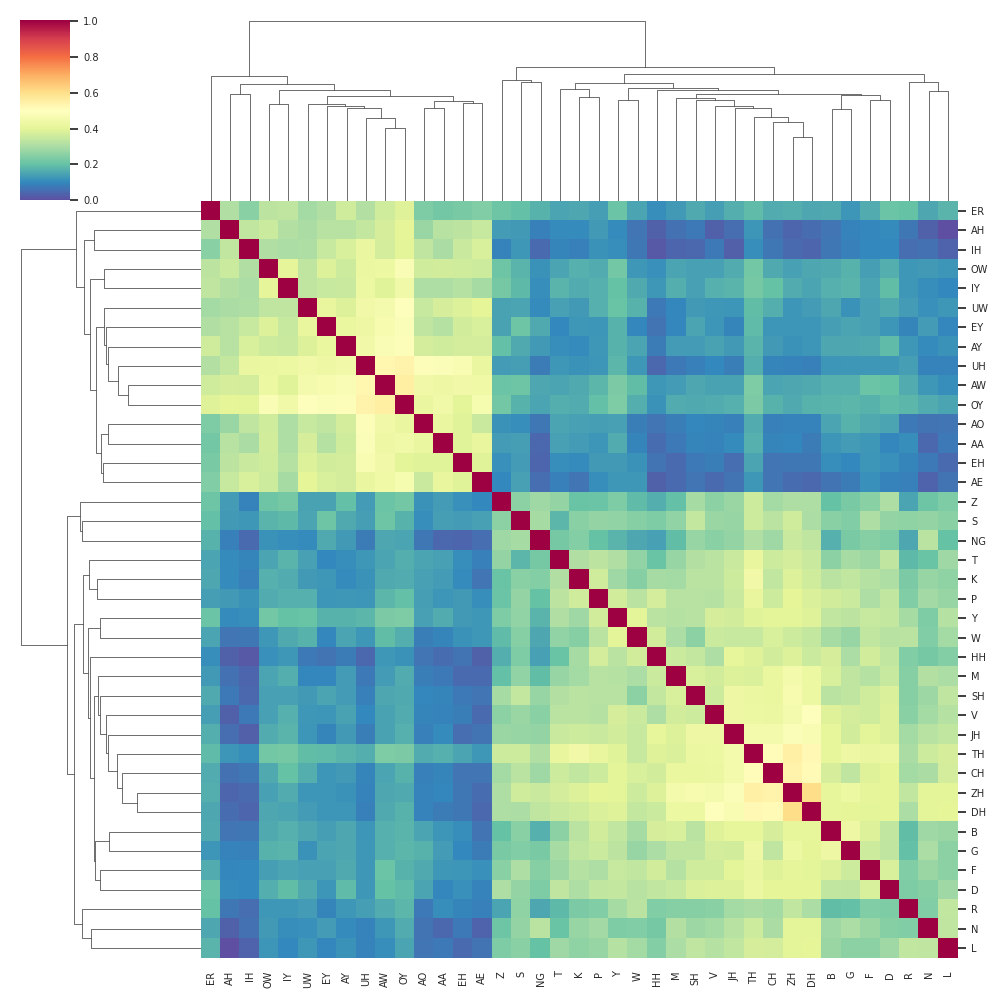
\includegraphics[scale=0.5]{phone-contextsimilarity.png}
    \caption{Phone classes of English based on Phonotactic similarity}
    \label{fig:contsim}
\end{figure}

The crucial take-home point from this discussion is the distinction between phonetics and phonotactics. While phonetics is concerned with the articulatory mechanisms of phone production, phonotactics is concerned with the contexts in which phones occur in a given language. Phonetics is language independent (for the most part although this is a simplification) while phonotactics can vary significantly across languages. For example, Spanish does not allow the fricative S in the word-initial position. Therefore, any English word starting with this consonant will be adapted to match the phonotactics of Spanish- the name `Steven' (/S T IY V AH N/) would be adapted to /EY S T EY B AA N/. Similarly, many languages have a phonological minimal word requirement. In the Dravidian language Telugu, the minimal word is a bimorac trochee, that is, it should consist of at least two moras and should be a trochee (stress on the initial of the two moras). In such a language, an English borrowing like the word 'bus' would be adapted to /B AH S S UH/. The vowel /EY/ in Spanish added word-initially to `Stephen' and the vowel /UH/ in Telugu added word-finally to `bus' are both instances of \textit{enunciative} vowel (also known as epenthetic vowel). This is like a gap-filler to adapt a foreign word to match the phonotactics of the native language. It is essential for engineers working on Speech technologies to read literature on phonetics-phonology and become familiar with these basic concepts in order to be able to build high quality models. Going back to the problems outlined at the start of the section, we can now see that the phone similarity approach needs to take into account both phonetic and phonotactic similarity when mapping phones across languages.

\section{Closing remarks and conclusion}

In this short article, I presented my arguments for why there needs to be a renewed engagement between researchers in linguistics and language technologies. I examined the similarity between the goals of lingustic theory and language technologies and argued that convergence between the two fields can not only be mutually beneficial but is essential. I presented a brief example of how lack of exposure to phonetics-phonology can make it hard to build high quality Speech technology. 

I conclude with the following thoughts-  
\begin{itemize}
    \item Does linguistics have all the answers about how Human Language works? Definitely not.
    \item Do current AI models cater to the complexity of linguistic phenomena? Absolutely not.
    \item Can linguists improve their theories by learning about AI and engineering? Definitely, see example of second law of thermodynamics. 
    \item Can engineers improve their models by learning about linguistic theories? Absolutely. A richer understanding of the linguistic signal will lead to more creative ways to pretrain neural language models. 
    
    \item Am I excited about future collaboration between linguistics and machine learning? Absolutely, definitely, most certainly.
\end{itemize}

\end{document}
